\chapter{Monte Carlo Methods}

Dynamic Programming (Chapter 3) requires full knowledge of the transition probability $P(s',r \mid s,a)$. In real-world problems (e.g., robotics, games, complex simulators), $P$ is unknown or too complex to explicitly sum over.

What we want is still $V^\pi(s)$: the \textbf{expected return} the agent gets from state $s$ if it follows policy $\pi$. That expectation depends on $\pi$ (which actions are chosen) and on the environment dynamics (where those actions lead and what rewards arrive). Without $P$, we cannot expand the expectation analytically.

$G_t$ scores one trajectory from time $t$. To observe it, the rest of that trajectory must be generated through to the end. That end is already in the setup: a terminal yields no further rewards, and (1.9) is the return when the run stops at a finite $T$. An \textbf{episode} is one such trajectory, from a start $S_0$ until termination (a terminal, or $T$). Take the taxi introduced in Chapter 1: it starts at a pickup, turns at junctions, and the run ends at drop-off. One realized episode is
\[
S_0{=}\text{pickup},\;
A_0{=}\text{left},\;
R_1{=}-1,\;
S_1{=}\text{junction},\;
A_1{=}\text{straight},\;
R_2{=}10,\;
S_2{=}\text{drop-off}
\quad\text{(terminal)}.
\]
The return from the pickup is $G_0=R_1+\gamma R_2=-1+10\gamma$, known only after drop-off. The next fare starts a new episode; it does not continue this sequence. So that next trip gives another $G_0$ from pickup, because what we want is the expected return $V^\pi(\text{pickup})$, not this one realized $G_0$. One episode is a sample; later episodes are further samples of the same expectation.

A state may occur more than once before termination. Those are multiple visits in the same episode, each with its own return from that time to the end; they are not multiple episodes. For example, the taxi may return to the same junction before drop-off; the extra loop is another visit, with more fuel cost in the reward.

Monte Carlo estimates $V^\pi$ by simulation: generate episodes under $\pi$, record the return $G_t$ from each visit to $s$, and average those returns. That average is the Monte Carlo estimator \eqref{eq:A.24} of \appref{A.4} for $V^\pi(s)=\mathbb{E}_\pi[G_t\mid S_t=s]$, which converges by the law of large numbers in \appref{A.3}. $G_t$ is known only when the episode has ended, so value updates are episode-by-episode (not step-by-step during the episode, as in TD later). A task that never terminates does not produce an episode in this sense, and Monte Carlo does not apply.

\section{First-Visit and Every-Visit}

A state may occur more than once in an episode. The taxi may return to the same junction before drop-off; that extra loop is a second visit, each with its own $G_t$ from that time to the end of the trip. Monte Carlo then has two possibilities for which of those returns enter the average.

\textbf{First-visit} keeps only the $G_t$ from the first time $s$ appears in the episode. \textbf{Every-visit} keeps the $G_t$ from every visit to $s$. Both estimate $V^\pi(s)=\mathbb{E}_\pi[G_t\mid S_t=s]$. First-visit averages one return per episode that hits $s$; every-visit averages the returns from all visits to $s$. With enough episodes, both converge to $V^\pi(s)$.

The same two rules apply to action-values: a visit is a pair $(s,a)$, first-visit keeps the return from the first time that pair appears in an episode, and every-visit keeps every occurrence. Both converge to $Q^\pi(s,a)$.

\begin{implnote}[Example ($\gamma=0.9$)]
Two episodes under $\pi$ (state-values only):

\begin{align*}
\text{Ep.~1:}\quad
&S_0{=}A
\xrightarrow{R_1{=}1}
S_1{=}B
\xrightarrow{R_2{=}0}
S_2{=}A
\xrightarrow{R_3{=}2}
S_3{=}C
\xrightarrow{R_4{=}3}
S_4{=}A
\xrightarrow{R_5{=}1}
S_5{=}D
\quad\text{(end)}.
\\[0.5em]
\text{Ep.~2:}\quad
&S_0{=}A
\xrightarrow{R_1{=}1}
S_1{=}B
\xrightarrow{R_2{=}2}
S_2{=}A
\xrightarrow{R_3{=}4}
S_3{=}D
\quad\text{(end)}.
\end{align*}

\begin{center}
\setlength{\tabcolsep}{7pt}%
\small
\begin{tabular}{lllll}
\toprule
$t$ &
\begin{tabular}{@{}l@{}}$S_t$\\[-0.15em]Ep.~1\end{tabular} &
\begin{tabular}{@{}l@{}}$G_t$\\[-0.15em]Ep.~1\end{tabular} &
\begin{tabular}{@{}l@{}}$S_t$\\[-0.15em]Ep.~2\end{tabular} &
\begin{tabular}{@{}l@{}}$G_t$\\[-0.15em]Ep.~2\end{tabular} \\
\midrule
$0$ & $A$ & $1+\gamma\cdot 0+\gamma^2\cdot 2+\gamma^3\cdot 3+\gamma^4\cdot 1=5.4631$ & $A$ & $1+\gamma\cdot 2+\gamma^2\cdot 4=6.04$ \\
$1$ & $B$ & $0+\gamma\cdot 2+\gamma^2\cdot 3+\gamma^3\cdot 1=4.959$ & $B$ & $2+\gamma\cdot 4=5.6$ \\
$2$ & $A$ & $2+\gamma\cdot 3+\gamma^2\cdot 1=5.51$ & $A$ & $4$ \\
$3$ & $C$ & $3+\gamma\cdot 1=3.9$ & $D$ & $0$ \\
$4$ & $A$ & $1$ &  &  \\
$5$ & $D$ & $0$ &  &  \\
\bottomrule
\end{tabular}
\end{center}

For $A$, first-visit keeps one return per episode ($5.4631$ from ep.\textasciitilde{}1, $6.04$ from ep.\textasciitilde{}2); every-visit keeps every visit return ($5.4631$, $5.51$, $1$ from ep.\textasciitilde{}1 and $6.04$, $4$ from ep.\textasciitilde{}2):

\[
\begin{aligned}
\text{first-visit:}\quad
&N(A)=2,\quad
V(A)=\frac{5.4631+6.04}{2}=5.75155
\\
\text{every-visit:}\quad
&N(A)=5,\quad
V(A)=\frac{5.4631+5.51+1+6.04+4}{5}=4.40262
\end{aligned}
\]
\end{implnote}

\section{State-value estimates}

The estimate of $V^\pi(s)=\mathbb{E}_\pi[G_t\mid S_t=s]$ is the average of the returns kept for $s$, first-visit or every-visit. After $N$ such returns $G^{(1)}(s),\ldots,G^{(N)}(s)$,

\begin{equation}
\begin{aligned}
V_N(s)
&=
\frac{1}{N}\sum_{i=1}^{N} G^{(i)}(s),
\\
\lim_{N\to\infty} V_N(s)
&=
\mathbb{E}_\pi[G_t \mid S_t=s]
=
V^\pi(s).
\end{aligned}
\tag{4.1}
\end{equation}

Here $N$ is the number of visits kept for $s$ (Section 4.1). Both first-visit and every-visit use (4.1); both converge as that $N\to\infty$.

We can update this sample mean \textbf{without} storing every past return. After $N$ returns the estimate is $V_N(s)$. When the next return $G^{(N+1)}(s)$ arrives:

\begin{equation}
\begin{aligned}
V_{N+1}(s)
&=
\frac{1}{N+1}\sum_{i=1}^{N+1} G^{(i)}(s)
\\
&=
\frac{1}{N+1}\Bigl( N\,V_N(s) + G^{(N+1)}(s) \Bigr)
\\
&=
V_N(s) + \frac{1}{N+1}\Bigl( G^{(N+1)}(s) - V_N(s) \Bigr).
\end{aligned}
\tag{4.2}
\end{equation}

So $V_N(s)$ summarizes the previous $N$ returns; the new return is folded in with weight $1/(N{+}1)$. Writing that weight as a step-size $\alpha$ gives

\begin{equation}
V_{N+1}(S_t)
\leftarrow
V_N(S_t) + \alpha \bigl( G_t^{(N+1)} - V_N(S_t) \bigr)
\tag{4.3}
\end{equation}

Here $t$ is the time in that episode, so $G_t=R_{t+1}+\gamma G_{t+1}$ is the return from the visit $S_t$, and $(N{+}1)$ is the next sample for that state.

If the policy $\pi$ and the environment $P$ are stationary, vary the step. After $N$ samples the next one is sample $n=N{+}1$; write $\alpha_{N+1}$ for the step on that sample. Then (4.3) is

\[
V_{N+1}(S_t)
\leftarrow
V_N(S_t) + \alpha_{N+1} \bigl( G_t^{(N+1)} - V_N(S_t) \bigr).
\]

Choose $\{\alpha_n\}$ so that

\[
\sum_{n=1}^{\infty}\alpha_n=\infty
\qquad\text{and}\qquad
\sum_{n=1}^{\infty}\alpha_n^2<\infty,
\]

as derived in \appref{D} (\citetxt{robbins1951}{Robbins and Monro, 1951}). One choice that meets both is $\alpha_n=1/n$, i.e.\ $\alpha_{N+1}=1/(N{+}1)$, which recovers (4.2). Then $V\to V^\pi$. First-visit and every-visit take \textbf{a fixed $\pi$} and do not update it, so they use (4.2).

If the target moves, as in typical RL (control: $\pi$ changes with $Q$), keep $\alpha$ in (4.3) fixed in $(0,1]$. A constant step does not meet $\sum\alpha_n^2<\infty$.

The first-visit and every-visit updates wait for the episode to end, then compute the returns from the last time back to the first. $G_t=R_{t+1}+\gamma G_{t+1}$ needs $G_{t+1}$ first, so start from $G\leftarrow 0$ at termination; at time $t$ that variable already holds $G_{t+1}$, and $G\leftarrow R_{t+1}+\gamma G$ produces $G_t$.

Each kept return is folded into $V$ inside the loop via (4.2): increment $N(s)$ first, then use weight $1/N(s)$---the same as dividing by $N_{\text{old}}+1$ before incrementing. That is equivalent to storing all returns and averaging once at the end, but without waiting and without keeping the full list. $N$ and $V$ persist across episodes. There is no fixed terminating condition. In theory we keep generating episodes indefinitely and (4.1) improves as $N\to\infty$; in practice stop after a chosen number of episodes, or when $V$ barely changes.

\textbf{First-visit} updates $V$ only when $S_t$ has not appeared earlier in that episode (at most once per state per episode).

\begin{implnote}[Algorithm (first-visit MC prediction for $V$)]
Input: $\pi$.

Output: $V\approx V^\pi$.

\begin{enumerate}
\item Initialize $V(s)$ arbitrarily and $N(s)\leftarrow 0$ for all $s$ (return count for $s$, not a global episode counter).
\item Loop forever (for each episode):
\begin{itemize}
\item Generate an episode following $\pi$:   $S_0,A_0,R_1,\;S_1,A_1,R_2,\;\ldots,\;S_{T-1},A_{T-1},R_T$.
\item $G\leftarrow 0$.
\item For $t=T{-}1,T{-}2,\ldots,0$:
\begin{itemize}
\item $G\leftarrow R_{t+1}+\gamma G$.
\item If $S_t\notin\{S_0,\ldots,S_{t-1}\}$ (first visit):
\begin{itemize}
\item $N(S_t)\leftarrow N(S_t)+1$,
\item $V(S_t)\leftarrow V(S_t)+\frac{1}{N(S_t)}\bigl(G-V(S_t)\bigr)$.
\end{itemize}
\end{itemize}
\end{itemize}
\item After enough episodes, return $V$ ($\approx V^\pi$).
\end{enumerate}

\end{implnote}

The same loop without that test. \textbf{Every-visit} updates $V$ on every visit to a state, not only the first (in the example of Section 4.1, episode 1 contributes $G_0$, $G_2$, and $G_4$ for $A$).

\begin{implnote}[Algorithm (every-visit MC prediction for $V$)]
Input: $\pi$.

Output: $V\approx V^\pi$.

\begin{enumerate}
\item Initialize $V(s)$ arbitrarily and $N(s)\leftarrow 0$ for all $s$.
\item Loop forever (for each episode):
\begin{itemize}
\item Generate an episode following $\pi$:   $S_0,A_0,R_1,\;S_1,A_1,R_2,\;\ldots,\;S_{T-1},A_{T-1},R_T$.
\item $G\leftarrow 0$.
\item For $t=T{-}1,T{-}2,\ldots,0$:
\begin{itemize}
\item $G\leftarrow R_{t+1}+\gamma G$.
\item $N(S_t)\leftarrow N(S_t)+1$,
\item $V(S_t)\leftarrow V(S_t)+\frac{1}{N(S_t)}\bigl(G-V(S_t)\bigr)$.
\end{itemize}
\end{itemize}
\item After enough episodes, return $V$ ($\approx V^\pi$).
\end{enumerate}

\end{implnote}

To implement the first-visit and every-visit algorithms for $V^\pi$ in Python, initialize the states, terminals, and actions, and define helpers that take one transition and generate an episode under $\pi$:

\lstinputlisting{../code/ch04/env_step.py}


The algorithms use that code. First-visit and every-visit for $V$ are:

\lstinputlisting{../code/ch04/mc_prediction_first_visit.py}


\section{Action-value estimates}

The same Monte Carlo idea applies to \textbf{action-values}. Recall $Q^\pi(s,a)=\mathbb{E}_\pi[G_t\mid S_t=s,A_t=a]$. A \textbf{visit} is now a pair $(s,a)$: after taking $a$ in $s$, record the return $G_t$ from that time and average. After $N$ such returns $G^{(1)}(s,a),\ldots,G^{(N)}(s,a)$,

\begin{equation}
\begin{aligned}
Q_N(s,a)
&=
\frac{1}{N}\sum_{i=1}^{N} G^{(i)}(s,a),
\\
\lim_{N\to\infty} Q_N(s,a)
&=
\mathbb{E}_\pi[G_t \mid S_t=s,A_t=a]
=
Q^\pi(s,a).
\end{aligned}
\tag{4.4}
\end{equation}

Here $N$ counts returns kept for that pair $(s,a)$ (first-visit: at most one per episode; every-visit: every occurrence of $(s,a)$). The incremental form of the sample mean is

\begin{equation}
\begin{aligned}
Q_{N+1}(s,a)
&=
Q_N(s,a) + \frac{1}{N+1}\Bigl( G^{(N+1)}(s,a) - Q_N(s,a) \Bigr).
\end{aligned}
\tag{4.5}
\end{equation}

With step-size $\alpha$ (the same two choices as after (4.3)), at a visit $(S_t,A_t)$ with return $G_t^{(N+1)}$,

\begin{equation}
Q_{N+1}(S_t,A_t)
\leftarrow
Q_N(S_t,A_t) + \alpha \bigl( G_t^{(N+1)} - Q_N(S_t,A_t) \bigr).
\tag{4.6}
\end{equation}

Compact code: $Q(S_t,A_t)\leftarrow Q(S_t,A_t)+\alpha\bigl(G_t-Q(S_t,A_t)\bigr)$.

The returns for $Q$ are computed the same way as for $V$, from the last time back to the first. First-visit updates $Q$ only on the first occurrence of $(S_t,A_t)$ in the episode; every-visit updates on every occurrence.

After $Q\approx Q^\pi$ is in hand, we may also return the greedy policy

\[
\pi'(s)=\arg\max_a Q(s,a).
\]

This $\pi'$ is greedy in $Q^\pi$, so it is an improvement of the $\pi$ that generated the episodes. It is $\pi^*$ only if that $\pi$ was already optimal. Here $\pi$ stays fixed while $Q$ is estimated. The evaluate--improve loop with $\pi\leftarrow\pi'$ is Section 4.4.

\begin{implnote}[Algorithm (first-visit MC prediction for $Q$)]
Input: $\pi$.

Output: $Q\approx Q^\pi$ and greedy $\pi'(s)=\arg\max_a Q(s,a)$.

\begin{enumerate}
\item Initialize $Q(s,a)$ arbitrarily and $N(s,a)\leftarrow 0$ for all $s,a$.
\item Loop forever (for each episode):
\begin{itemize}
\item Generate an episode following $\pi$:   $S_0,A_0,R_1,\;\ldots,\;S_{T-1},A_{T-1},R_T$.
\item $G\leftarrow 0$.
\item For $t=T{-}1,\ldots,0$:
\begin{itemize}
\item $G\leftarrow R_{t+1}+\gamma G$.
\item If $(S_t,A_t)$ is a first visit in this episode:
\begin{itemize}
\item $N(S_t,A_t)\leftarrow N(S_t,A_t)+1$,
\item $Q(S_t,A_t)\leftarrow Q(S_t,A_t)+\frac{1}{N(S_t,A_t)}\bigl(G-Q(S_t,A_t)\bigr)$.
\end{itemize}
\end{itemize}
\end{itemize}
\item For each $s$, set $\pi'(s)=\arg\max_a Q(s,a)$. Return $Q$ and $\pi'$.
\end{enumerate}

\end{implnote}

\textbf{Every-visit} updates $Q$ on every occurrence of $(S_t,A_t)$, not only the first.

\begin{implnote}[Algorithm (every-visit MC prediction for $Q$)]
Input: $\pi$.

Output: $Q\approx Q^\pi$ and greedy $\pi'(s)=\arg\max_a Q(s,a)$.

\begin{enumerate}
\item Initialize $Q(s,a)$ and $N(s,a)\leftarrow 0$ as above.
\item Loop forever (for each episode):
\begin{itemize}
\item Generate an episode following $\pi$.
\item $G\leftarrow 0$.
\item For $t=T{-}1,\ldots,0$:
\begin{itemize}
\item $G\leftarrow R_{t+1}+\gamma G$.
\item $N(S_t,A_t)\leftarrow N(S_t,A_t)+1$,
\item $Q(S_t,A_t)\leftarrow Q(S_t,A_t)+\frac{1}{N(S_t,A_t)}\bigl(G-Q(S_t,A_t)\bigr)$.
\end{itemize}
\end{itemize}
\item For each $s$, set $\pi'(s)=\arg\max_a Q(s,a)$. Return $Q$ and $\pi'$.
\end{enumerate}

\end{implnote}

The toy environment of Section 4.2 is reused here. First-visit and every-visit for $Q$, with a greedy readout $\pi'$, are:

\lstinputlisting{../code/ch04/mc_q_prediction.py}


\section{Monte Carlo Control}

Sections 4.2--4.3 are prediction: $V^\pi$ or $Q^\pi$ for a given $\pi$, from episode returns, without $P$. This section is control: a policy that is (approximately) optimal in every state,

\[
\pi^*
\in
\arg\max_\pi V^\pi(s)
\quad\text{for every }s
\]

(equivalently, act greedily on $Q^*$).

In Sections 4.2--4.3 the input $\pi$ is \textbf{fixed}: every episode is generated under that same $\pi$, and only $V$ or $Q$ is updated. More episodes refine $Q\to Q^\pi$ (better values for \textbf{that} $\pi$), but the behavior policy never changes. Section 4.3 may return a greedy readout

\begin{equation}
\pi'(s)=\arg\max_a Q(s,a)
\tag{4.7}
\end{equation}

after $Q$ is estimated; that $\pi'$ is taken from the finished table, not used to generate further episodes. So prediction improves the value estimates under a fixed policy---and can propose an improved $\pi'$---yet never updates the policy that collects data.

The gap for control is exactly that missing update of $\pi$. The fix is to run an \textbf{evaluate--improve} cycle: estimate $Q$ for the current $\pi$ by Monte Carlo ((4.4)--(4.6), as in Section 4.3), then replace $\pi$ by the greedy policy (4.7), then evaluate again under the new $\pi$, and so on until $\pi$ stops changing. Improve can wait until $Q$ has settled for the current $\pi$ (many episodes), or run after every episode---same Improve step, only a different schedule.

The $Q$ update in that cycle is still the sample mean (4.5), with weight $1/N$. The environment $P$ is unchanged; only $\pi$ changes, so the i.i.d.\ returns assumed in \appref{D} do not hold while Improve is still moving $\pi$. A constant $\alpha$, as after (4.3), never meets $\sum\alpha_n^2<\infty$, so $Q$ keeps moving and the greedy $\pi$ can keep flipping. The $1/N$ step is kept so that $Q$ can settle. In practice that freeze of $\pi$ happens after some episodes (Figure~\ref{fig-4-1}); Robbins--Monro then applies to the remaining $1/k$ steps.

\begin{figure}[ht]
\centering
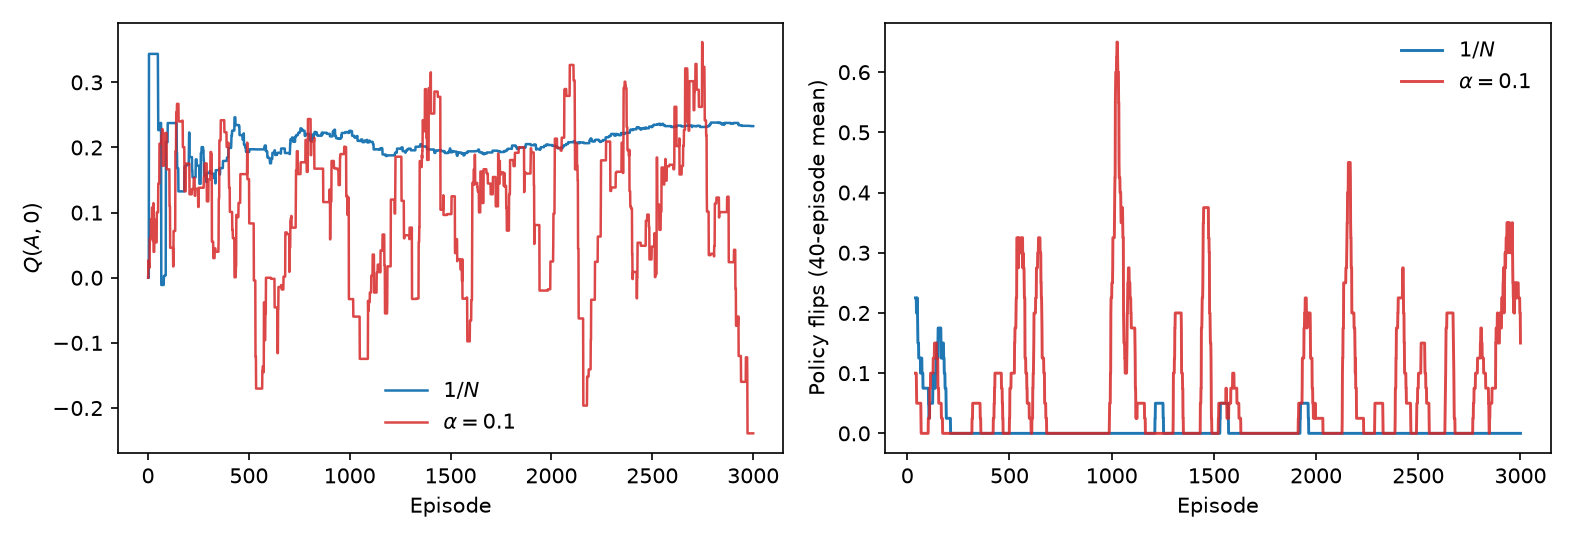
\includegraphics[width=\textwidth]{mc_es_step_size.png}
\caption{Monte Carlo ES, $1/N$ versus $\alpha=0.1$. Left: $Q(A,0)$. Right: greedy-action flips (40-episode mean).}
\label{fig-4-1}
\end{figure}

A bare skeleton is:

\begin{implnote}[Algorithm (Monte Carlo control skeleton)]
Input: none (episodes generated under the current $\pi$).

Output: $Q$ and $\pi$.

\begin{enumerate}
\item Initialize $\pi$ arbitrarily. Initialize $Q(s,a)$ arbitrarily and $N(s,a)\leftarrow 0$.
\item \textbf{Evaluate.} Generate episodes by following the current $\pi$. Update $Q$ by first- or every-visit Monte Carlo averaging of returns (until $Q$ has settled for this $\pi$, or after each episode).
\item \textbf{Improve.} For each $s$, set $\pi(s)\leftarrow\arg\max_a Q(s,a)$.
\item If $\pi$ changed, go to step 2. Otherwise return $Q$ and $\pi$.
\end{enumerate}

\end{implnote}

The skeleton has a problem in Evaluate. Episodes follow the current $\pi$, so $Q$ is updated only for actions $\pi$ actually takes. After Improve, $\pi$ is greedy on $Q$: at each state it picks the single action $\pi(s)=\arg\max_a Q(s,a)$. The next Evaluate then follows that greedy $\pi$ again---so other actions are never tried, their $Q$ entries never improve, and Improve cannot switch to them. The loop can get stuck on a poor policy even though a better action exists.

To get every action tried often enough, change how episodes are generated---and, if needed, how Improve updates $\pi$. This can be done with \textbf{on-policy} or \textbf{off-policy} methods. An on-policy method evaluates and improves the \textbf{same} policy that generates the decisions (and thus the episodes). An off-policy method learns about one policy (the \textbf{target}) while generating data with a different exploring policy (the \textbf{behavior}). Three standard Monte Carlo methods are exploring starts, $\varepsilon$-greedy policies, and off-policy Monte Carlo. The first two are on-policy; the third is off-policy.

\subsection{Exploring starts}

In the skeleton, Improve sets $\pi(s)=\arg\max_a Q(s,a)$, so Evaluate always starts with the same action at $S_0$: $A_0=\pi(S_0)$. Exploring starts replace that first choice by drawing $(S_0,A_0)$ from a distribution that puts positive probability on every pair (e.g. uniform), \textbf{not} from $\pi$; then follow $\pi$ from $S_1$ onward and update $Q$ as usual. That draw is not possible if every episode must begin at a fixed $S_0$ with $A_0=\pi(S_0)$. Improve stays greedy as in the skeleton: $\pi(s)\leftarrow\arg\max_a Q(s,a)$. From $S_1$ the episode follows that $\pi$, so Evaluate and Improve are on the same policy that generates those later actions, and the method is on-policy.
\begin{implnote}[Algorithm (Monte Carlo ES)]
Input: start distribution over $(s,a)$ with positive probability on every pair.

Output: $Q\approx Q^*$ and $\pi\approx\pi^*$.

\begin{enumerate}
\item Initialize $Q(s,a)$ arbitrarily, $N(s,a)\leftarrow 0$, and $\pi$ arbitrarily (e.g. random or greedy on $Q$).
\item Loop forever (each episode):
\begin{itemize}
\item Draw $(S_0,A_0)$ from a distribution over $\mathcal{S}\times\mathcal{A}$ that puts positive probability on every pair (e.g. uniform).
\item Generate the rest of the episode by following $\pi$: $S_0,A_0,R_1,\ldots,S_{T-1},A_{T-1},R_T$.
\item $G\leftarrow 0$. For $t=T{-}1,\ldots,0$:
\begin{itemize}
\item $G\leftarrow R_{t+1}+\gamma G$.
\item If $(S_t,A_t)$ is a first visit in this episode:
\begin{itemize}
\item $N(S_t,A_t)\leftarrow N(S_t,A_t)+1$,
\item $Q(S_t,A_t)\leftarrow Q(S_t,A_t)+\frac{1}{N(S_t,A_t)}\bigl(G-Q(S_t,A_t)\bigr)$.
\end{itemize}
\end{itemize}
\item For each $s$ appearing in the episode: $\pi(s)\leftarrow\arg\max_a Q(s,a)$.
\end{itemize}
\item After enough episodes (or when $\pi$ stops changing), return $Q$ and $\pi$ ($\approx Q^*$, $\approx\pi^*$).
\end{enumerate}

\end{implnote}

The environment of Section 4.2 is reused here. Exploring starts needs its own episode generator:

\lstinputlisting{../code/ch04/mc_es.py}


\subsection{$\varepsilon$-greedy policies}

Another way to try every action is to select with probability instead of always taking the greedy action. Unlike exploring starts, $A_0$ and the following actions are chosen by $\pi$. The greedy action in $Q$ is $A^*=\arg\max_a Q(s,a)$. If Improve set $\pi(s)=A^*$ as in exploring starts, that action would be locked. Therefore, instead of $\pi(s)=A^*$, Improve changes $\pi$ so that $A^*$ is taken with probability $1-\varepsilon$ and otherwise (probability $\varepsilon$) an action is chosen uniformly from $\mathcal{A}$ (the greedy action could also be picked). That selection rule is the policy $\pi$. Evaluate generates every $A_t$ from that same $\pi$. Because we act and learn with the same $\varepsilon$-greedy $\pi$, this is on-policy. The loop aims at the best such exploring policy; driving $\varepsilon\to 0$ carefully recovers a near-greedy optimum. This is the usual practical default.
\begin{implnote}[Algorithm (on-policy first-visit MC control, $\varepsilon$-greedy)]
Input: $\varepsilon\in(0,1]$.

Output: $Q\approx Q^*$ and greedy $\pi\approx\pi^*$ (for acting); learning uses an $\varepsilon$-greedy behavior.

\begin{enumerate}
\item Initialize $Q(s,a)$ arbitrarily, $N(s,a)\leftarrow 0$, and behavior $\pi$ as an arbitrary $\varepsilon$-greedy policy.
\item Loop forever (each episode):
\begin{itemize}
\item Generate an episode by following $\pi$: $S_0,A_0,R_1,\ldots,R_T$.
\item $G\leftarrow 0$. For $t=T{-}1,\ldots,0$:
\begin{itemize}
\item $G\leftarrow R_{t+1}+\gamma G$.
\item If $(S_t,A_t)$ is a first visit in this episode:
\begin{itemize}
\item $N(S_t,A_t)\leftarrow N(S_t,A_t)+1$,
\item $Q(S_t,A_t)\leftarrow Q(S_t,A_t)+\frac{1}{N(S_t,A_t)}\bigl(G-Q(S_t,A_t)\bigr)$.
\end{itemize}
\end{itemize}
\item For each $s$ appearing in the episode:
\begin{itemize}
\item $A^*\leftarrow\arg\max_a Q(s,a)$,
\item set $\pi(\,\cdot\mid s)$ $\varepsilon$-greedy on $A^*$: probability $1-\varepsilon+\varepsilon/|\mathcal{A}|$ on $A^*$, and $\varepsilon/|\mathcal{A}|$ on every other action.
\end{itemize}
\end{itemize}
\item After enough episodes, return $Q$ and the greedy policy $\pi'(s)=\arg\max_a Q(s,a)$ as the estimate of $\pi^*$ (keep $\varepsilon$-greedy $\pi$ only while learning).
\end{enumerate}

\end{implnote}

The environment of Section 4.2 is reused here, and \texttt{greedy\_pi} from Section 4.3. On-policy $\varepsilon$-greedy control is:

\lstinputlisting{../code/ch04/on_policy_mc_control.py}


\subsection{Off-policy Monte Carlo}

In the methods above, the same policy both \textbf{acts} and is \textbf{evaluated}. Off-policy learning splits that role. A \textbf{behavior} policy $b$ generates the episodes (and must keep exploring, e.g. $\varepsilon$-greedy). A \textbf{target} policy $\pi$ is the policy whose action-values we estimate. In this section that $\pi$ is greedy on $Q$: $\pi(s)=\arg\max_a Q(s,a)$. The question is how to estimate $Q^\pi$ when every sample comes from $b$. \textbf{Importance sampling} does that: it estimates an expectation under a target distribution $p$ from samples drawn from a \textbf{proposal} distribution $q$, by reweighting each sample with $p/q$.

The idea of importance sampling (derived in \appref{A}) is to rewrite an expectation under a target distribution $p$ using samples from a proposal distribution $q$:

\[
\mathbb{E}_{x\sim p}[f(x)]
=
\mathbb{E}_{x\sim q}\bigl[w(x)\, f(x)\bigr],
\qquad
w(x)=\frac{p(x)}{q(x)}.
\]

Two forms approximate that expectation from draws $x_i\sim q$---\textbf{ordinary} and \textbf{weighted} importance sampling (see \appref{A}):

\[
\mathbb{E}_{x\sim p}[f(x)]
\approx
\frac{1}{N}\sum_{i=1}^{N} w(x_i)\, f(x_i),
\]

\[
\mathbb{E}_{x\sim p}[f(x)]
\approx
\frac{\sum_{i=1}^{N} w(x_i)\, f(x_i)}{\sum_{i=1}^{N} w(x_i)}.
\]

Here each sample $x$ will be a \textbf{trajectory}; $N$ is the number of such trajectory samples.

For action-values under the target policy,

\begin{equation}
Q^\pi(s,a)
=
\mathbb{E}_\pi[G_t\mid S_t=s,A_t=a].
\tag{4.8}
\end{equation}

An episode generated by the behavior $b$ always starts at $t=0$:

\[
S_0,A_0,R_1,S_1,\ldots,S_{T-1},A_{T-1},R_T.
\]

A trajectory from time $t$, given $S_t$, is

\[
A_t,R_{t+1},S_{t+1},A_{t+1},R_{t+2},\ldots,A_{T-1},R_T.
\]

This is the sample $x$ in the importance-sampling formulas above. The same episode can contain the pair $(S_t,A_t)=(s,a)$ more than once; each occurrence starts its own trajectory sample. The return

\[
G_t=R_{t+1}+\gamma R_{t+2}+\cdots+\gamma^{T-t-1}R_T
\]

is a function of this trajectory ($f(x)=G_t$). Under a policy $\pi$, the probability of the trajectory given $S_t$ is (chain rule; environment factors written as $P(s',r\mid s,a)$)

\[
\begin{aligned}
&P_\pi(A_t,R_{t+1},S_{t+1},\ldots,R_T\mid S_t)
\\
&\quad=
\prod_{k=t}^{T-1}
\pi(A_k\mid S_k)\,
P(S_{k+1},R_{k+1}\mid S_k,A_k).
\end{aligned}
\]

The same expansion under $b$ replaces each $\pi$ by $b$. The importance-sampling weight from the opening of this subsection is their ratio (require $b(a\mid s)>0$ whenever $\pi(a\mid s)>0$):

\begin{equation}
w
=
\rho_{t:T-1}
:=
\frac{P_\pi(A_t,R_{t+1},S_{t+1},\ldots,R_T\mid S_t)}{P_b(A_t,R_{t+1},S_{t+1},\ldots,R_T\mid S_t)}.
\tag{4.9}
\end{equation}

Those environment factors do not depend on the policy: the same $P(S_{k+1},R_{k+1}\mid S_k,A_k)$ appears in $P_\pi$ and in $P_b$. They cancel, so

\[
\rho_{t:T-1}
=
\prod_{k=t}^{T-1}
\frac{\pi(A_k\mid S_k)}{b(A_k\mid S_k)}.
\]

Apply importance sampling \eqref{eq:A.13} to (4.8): the target is $\pi$, the proposal is $b$, the weight is (4.9), and $f=G_t$. Then

\begin{equation}
Q^\pi(s,a)
=
\mathbb{E}_b\bigl[\rho_{t:T-1}\,G_t\mid S_t=s,A_t=a\bigr].
\tag{4.10}
\end{equation}

With $N$ trajectory samples from visits to $(s,a)$ under $b$---each sample $x_i$ the trajectory from that visit, with return $G^{(i)}$ and weight $\rho^{(i)}=\rho_{t:T-1}^{(i)}$---ordinary and weighted importance sampling give

\begin{equation}
Q(s,a)
\approx
\frac{1}{N}\sum_{i=1}^{N}\rho^{(i)}G^{(i)},
\tag{4.11}
\end{equation}

\begin{equation}
Q(s,a)
\approx
\frac{\sum_{i=1}^{N}\rho^{(i)}G^{(i)}}{\sum_{i=1}^{N}\rho^{(i)}}.
\tag{4.12}
\end{equation}

Write $Q_N(s,a)$ for the weighted estimate (4.12). When visit $N{+}1$ brings $G^{(N+1)}(s,a)$ and $\rho^{(N+1)}(s,a)$,

\begin{equation}
Q_{N+1}(s,a)
=
Q_N(s,a)
+
\frac{\rho^{(N+1)}}{\sum_{i=1}^{N+1} \rho^{(i)}}
\Bigl(
G^{(N+1)}(s,a) - Q_N(s,a)
\Bigr).
\tag{4.13}
\end{equation}

To apply (4.13) episode by episode, walk each episode \textbf{backward} ($t=T{-}1,\ldots,0$), as in Section 4.2. Start from $G\leftarrow 0$ and $\rho\leftarrow 1$: that is $G_T=0$ (no rewards after termination) and $\rho_{T:T-1}=1$ (empty product).

At each $t$ while $\rho\neq 0$: form $G_t$ by $G\leftarrow R_{t+1}+\gamma G$, apply (4.13) with the current $\rho$ ($C(s,a)$ stores $\sum_i\rho^{(i)}$), set $\pi(S_t)\leftarrow\arg\max_a Q(S_t,a)$, then $\rho\leftarrow\rho\cdot\pi(A_t\mid S_t)/b(A_t\mid S_t)$. Here $\pi$ is deterministic: it puts probability $1$ on its chosen action at $S_t$ and $0$ on every other action. So if behavior selected $A_t$, then $\pi(A_t\mid S_t)=1$ only when that $A_t$ is $\pi$'s action, and $0$ otherwise. When that factor is $0$, $\rho$ becomes $0$ and the loop stops---further multiplications for earlier times $t{-}1,t{-}2,\ldots$ would leave $\rho$ at $0$.

The behavior $b$ may be any policy. The only requirement is coverage of $\pi$: $b(a\mid s)>0$ whenever $\pi(a\mid s)>0$. Soft or $\varepsilon$-greedy policies always guarantee that, so the denominator of $\rho$ stays positive and a zero $\rho$ comes only from $\pi(A_t\mid S_t)$.

\begin{implnote}[Algorithm (off-policy MC control, weighted importance sampling)]
Input: behavior $b$ with coverage for $\pi$ (e.g. $\varepsilon$-greedy on $Q$).

Output: $Q\approx Q^*$ and greedy $\pi\approx\pi^*$.

\begin{enumerate}
\item Initialize $Q(s,a)$ arbitrarily and $C(s,a)\leftarrow 0$.
\item Loop forever (each episode):
\begin{itemize}
\item $b\leftarrow$ any policy with coverage for $\pi$: $b(a\mid s)>0$ whenever $\pi(a\mid s)>0$ (soft or $\varepsilon$-greedy $b$ always guarantees coverage).
\item Generate an episode by following $b$: $S_0,A_0,R_1,\ldots,S_{T-1},A_{T-1},R_T$.
\item $G\leftarrow 0$, $\rho\leftarrow 1$.
\item For $t=T{-}1,\ldots,0$ while $\rho\neq 0$:
\begin{itemize}
\item $G\leftarrow R_{t+1}+\gamma G$.
\item $C(S_t,A_t)\leftarrow C(S_t,A_t)+\rho$,
\item $Q(S_t,A_t)\leftarrow Q(S_t,A_t)+\frac{\rho}{C(S_t,A_t)}\bigl(G-Q(S_t,A_t)\bigr)$.
\item $\pi(S_t)\leftarrow\arg\max_a Q(S_t,a)$.
\item $\rho\leftarrow\rho\cdot\frac{\pi(A_t\mid S_t)}{b(A_t\mid S_t)}$ ($\pi$ puts probability $1$ on its action at $S_t$ and $0$ on all others; so $\pi(A_t\mid S_t)=1$ if behavior's $A_t$ is that action, else $0$).
\end{itemize}
\end{itemize}
\item After enough episodes, return $Q$ and the greedy $\pi(s)=\arg\max_a Q(s,a)$ ($\approx Q^*$, $\approx\pi^*$).
\end{enumerate}

\end{implnote}

The environment of Section 4.2 is reused here, and \texttt{eps\_greedy} and \texttt{generate\_episode} from Section 4.4.2. Off-policy control is:

\lstinputlisting{../code/ch04/off_policy_mc_control.py}


\subsubsection*{Off-policy state-values}

The same importance-sampling argument gives state-values. With $V^\pi(s)=\mathbb{E}_\pi[G_t\mid S_t=s]$ and the same weight (4.9),

\begin{equation}
V^\pi(s)
=
\mathbb{E}_b\bigl[\rho_{t:T-1}\,G_t\mid S_t=s\bigr].
\tag{4.14}
\end{equation}

With $N$ trajectory samples from visits to $s$ under $b$, returns $G^{(i)}$, and weights $\rho^{(i)}=\rho_{t:T-1}^{(i)}$, ordinary and weighted importance sampling give

\begin{equation}
V(s)
\approx
\frac{1}{N}\sum_{i=1}^{N}\rho^{(i)}G^{(i)},
\tag{4.15}
\end{equation}

\begin{equation}
V(s)
\approx
\frac{\sum_{i=1}^{N}\rho^{(i)}G^{(i)}}{\sum_{i=1}^{N}\rho^{(i)}}.
\tag{4.16}
\end{equation}

Write $V_N(s)$ for the weighted estimate (4.16). When visit $N{+}1$ brings $G^{(N+1)}(s)$ and $\rho^{(N+1)}(s)$,

\begin{equation}
V_{N+1}(s)
=
V_N(s)
+
\frac{\rho^{(N+1)}}{\sum_{i=1}^{N+1} \rho^{(i)}}
\Bigl(
G^{(N+1)}(s) - V_N(s)
\Bigr).
\tag{4.17}
\end{equation}
